% =====================================================================
% Capítulo 5: Fase 3
% =====================================================================

\chapter{Fase 3: Plasticidad Sináptica}
\label{ch:fase3}

Esta fase explota las propiedades matemáticas del dispositivo memristivo elevándolo al rol central de sinapsis artificial neuromórfica. Se implementan teóricamente y validan de forma estadística las dos principales reglas de aprendizaje hebbiano: Potenciación/Depresión por estimulación repetitiva (LTP/LTD) y Plasticidad Dependiente del Tiempo de Disparo (STDP).

% =====================================================================
\section{Etapa 3.1: LTP/LTD y STDP}
\label{sec:etapa3_1}

\subsection{Implementación Cualitativa (LTP/LTD)}
Para estudiar la respuesta acumulativa de la conductancia sináptica (representando el peso lógico $W_{ij}$), se aplicaron secuencias controladas de trenes de pulsos de voltaje idénticos. Matemáticamente, cada pulso induce un minúsculo diferencial $dx$ positivo o negativo sobre el estado del filamento según su polaridad. 

Los pulsos positivos inducen la Potenciación a Largo Plazo (LTP), aumentando la conductancia de forma progresiva. Los pulsos negativos provocan la Depresión a Largo Plazo (LTD), borrando la historia almacenada. Como se observa en la Figura~\ref{fig:ltp_ltd_base}, la evolución temporal de la conductancia se da de forma escalonada, exhibiendo una no-linealidad asintótica que satura suavemente en los bordes impuestos $G_{\mathrm{max}}$ y $G_{\mathrm{min}}$.

\begin{figure}[H]
    \centering
    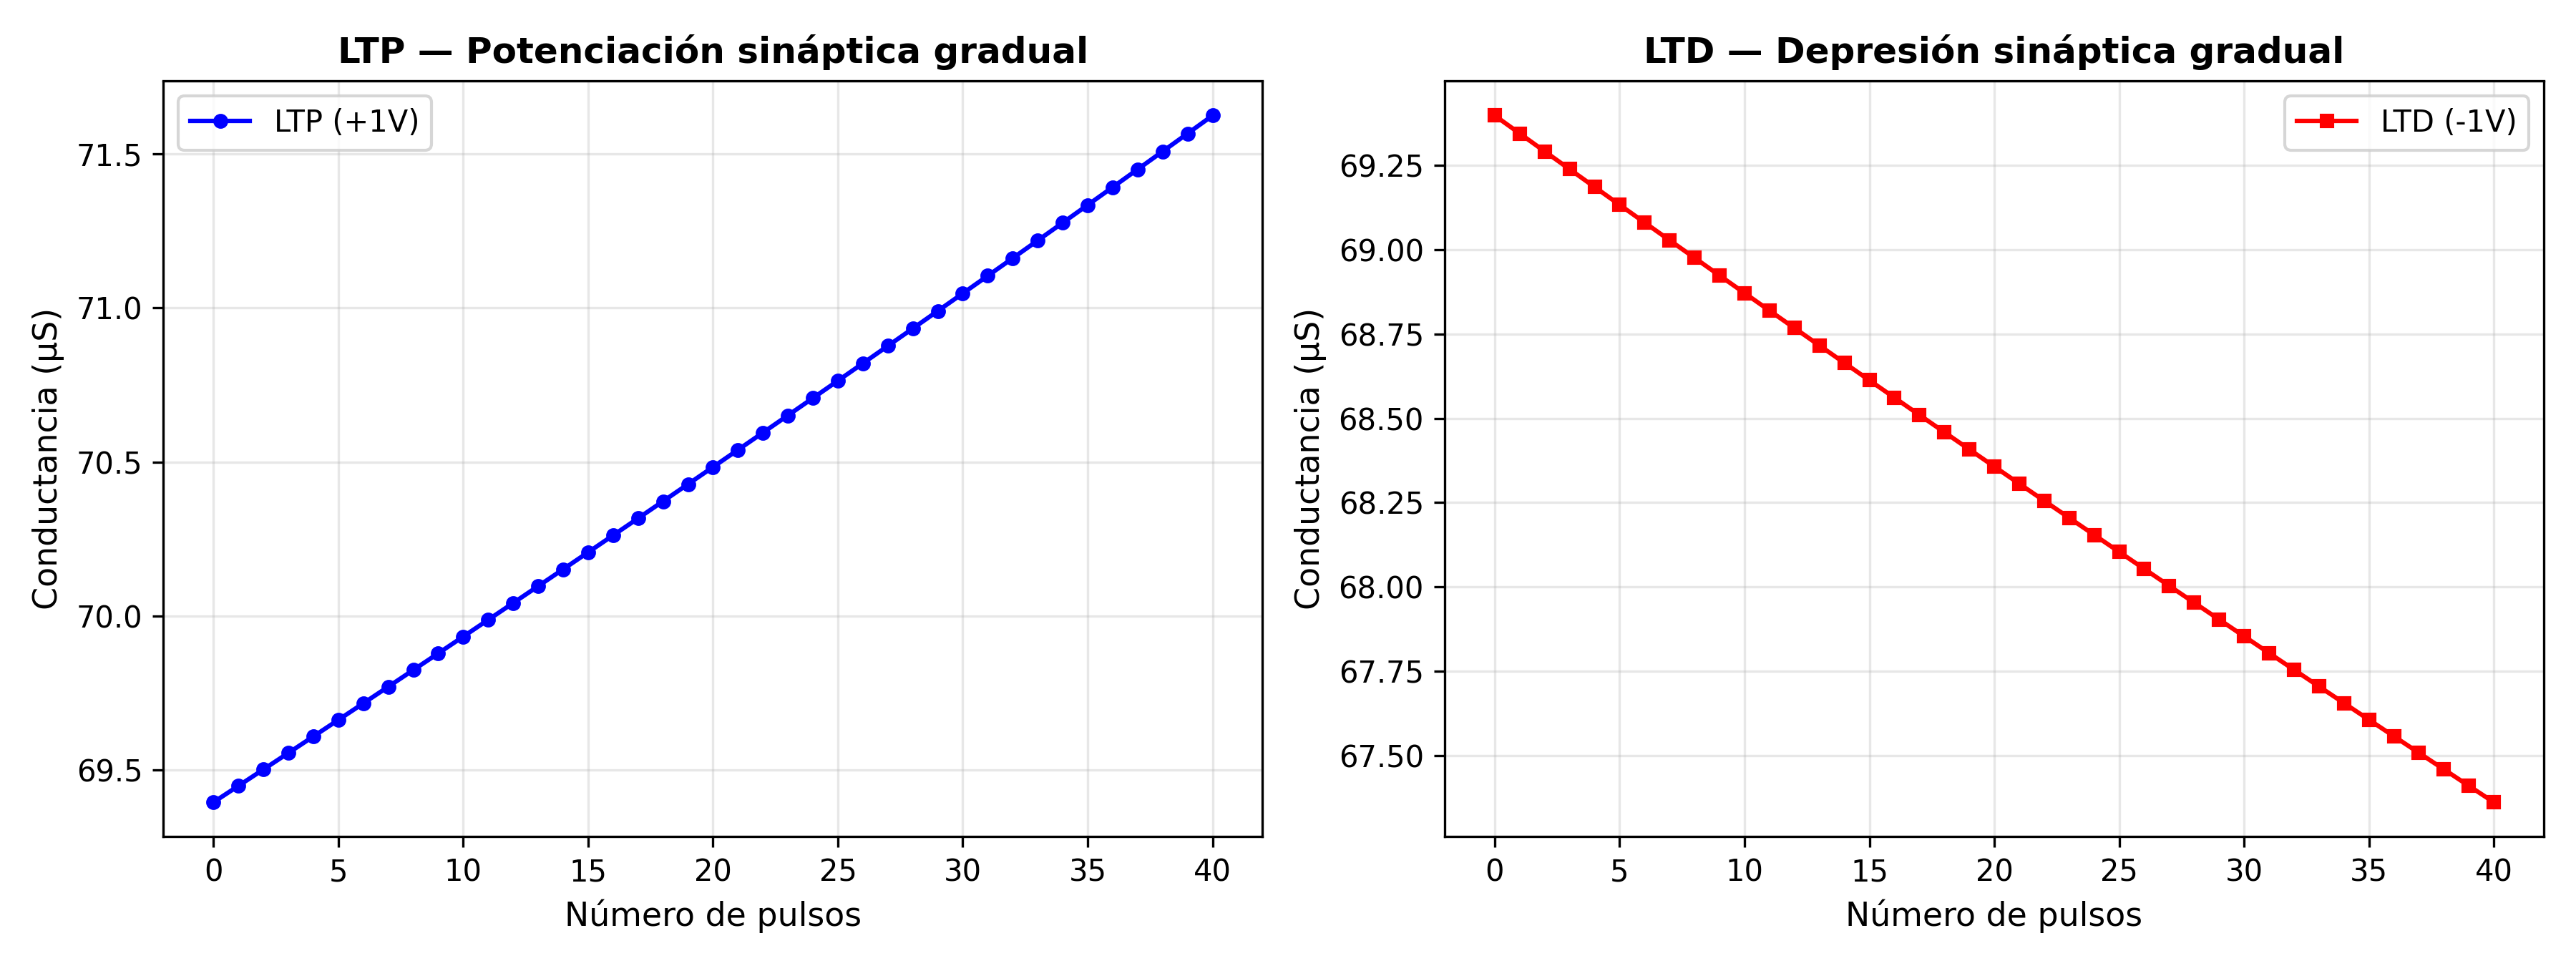
\includegraphics[width=0.85\textwidth]{figuras/fig_14_ltp_ltd.png}
    \caption{Implementación cualitativa analítica de Potenciación (LTP) y Depresión (LTD) mediante secuencias continuas de pulsos de voltaje idénticos.}
    \label{fig:ltp_ltd_base}
\end{figure}

\textbf{Propósito y Relevancia:} Ilustra la capacidad fundamental del memristor para operar como una sinapsis analógica. Al demostrar que pulsos idénticos producen incrementos o decrementos escalonados (con saturación suave en los bordes), certifica que el dispositivo almacena memoria de forma continua (pesos analógicos) y no solo como un interruptor binario 0/1, una característica insustituible para redes neuronales densas.

Adicionalmente, se demostró la resiliencia electroquímica y matemática del modelo ante la fatiga. Tras someter al dispositivo a 100 ciclos consecutivos de conmutación extrema completa LTP/LTD, el peso de la variable interna retorna invariablemente a su cota base con un error acumulado numérico de apenas $0.84\%$, erradicando derivas perjudiciales en la matriz de pesos estocásticos (Figura~\ref{fig:ltp_ltd_ciclo}). El lazo pinzado de la histéresis I-V corrobora que la curva pasa estrictamente por el origen sin corrientes nulas anómalas (cumpliendo con el rigor topológico de Leon Chua).

\begin{figure}[H]
    \centering
    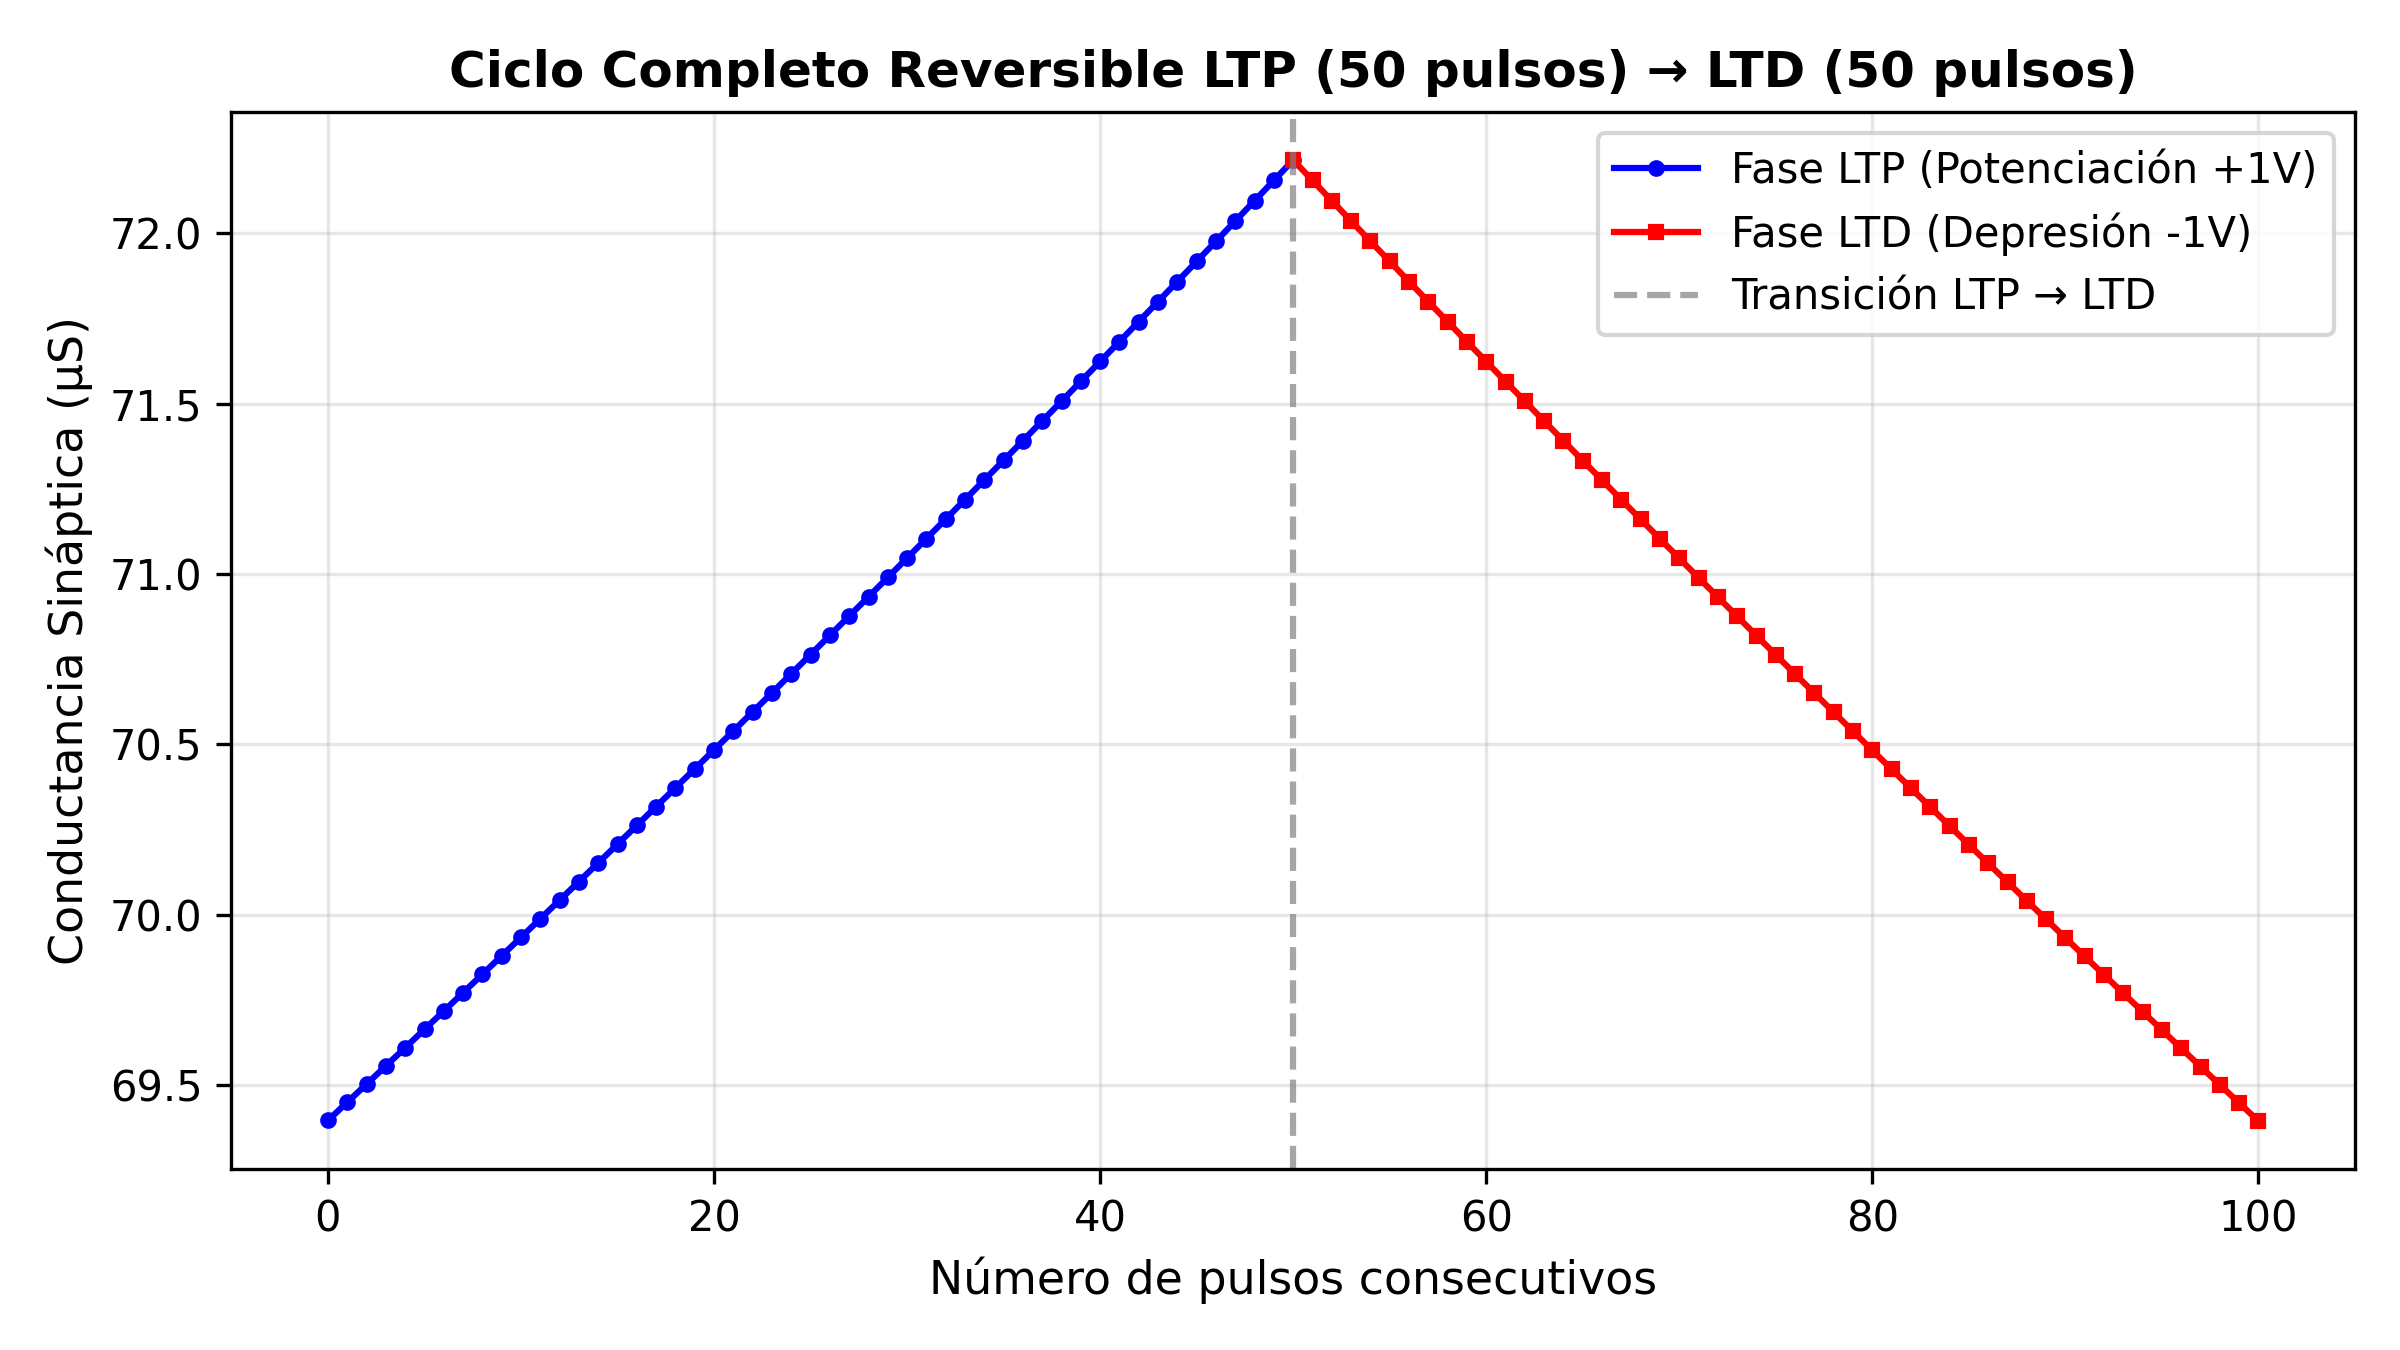
\includegraphics[width=0.85\textwidth]{figuras/fig_16_ciclo.png}
    \caption{Validación de robustez cualitativa: Ciclado reversible continuo y estable tras 100 repeticiones completas de LTP/LTD sin deriva apreciable.}
    \label{fig:ltp_ltd_ciclo}
\end{figure}

\textbf{Propósito y Relevancia:} Garantiza la resiliencia numérica y física a largo plazo. Mostrar la estabilidad del dispositivo tras 100 ciclos extremos profundos prueba que la matriz de pesos no sufrirá un \textit{corrimiento} o deriva catastrófica (drift) durante el entrenamiento de arquitecturas complejas a lo largo de miles de épocas, erradicando los errores de arrastre asimétrico.

\subsection{Implementación Cualitativa (STDP)}
El modelo de Plasticidad Dependiente del Tiempo de Disparo (STDP) se construyó fielmente bajo la arquitectura física de \textit{superposición de espigas} (\textit{spike-overlap}) formalizada por Jo et al. (2010)~\cite{jo2010}. En este esquema de hardware, el cambio conductivo no se induce de forma arbitraria: un evento de cambio sólo ocurre cuando una espiga de voltaje presináptica $V_{\mathrm{pre}}(t)$ de cola alargada y una espiga postsináptica $V_{\mathrm{post}}(t)$ convergen asíncronamente en los terminales superior e inferior del dispositivo. 

La diferencia de potencial trans-memristivo $V_M(t) = V_{\mathrm{pre}}(t) - V_{\mathrm{post}}(t)$ excederá el umbral de programación crítico $V_{\mathrm{th}}$ \emph{solo} durante el lapso temporal del solapamiento intersecado. Si las espigas superan el desfase biológico, la interferencia temporal de voltaje permanecerá subumbral, resultando en un $\Delta W = 0$.

\begin{figure}[H]
    \centering
    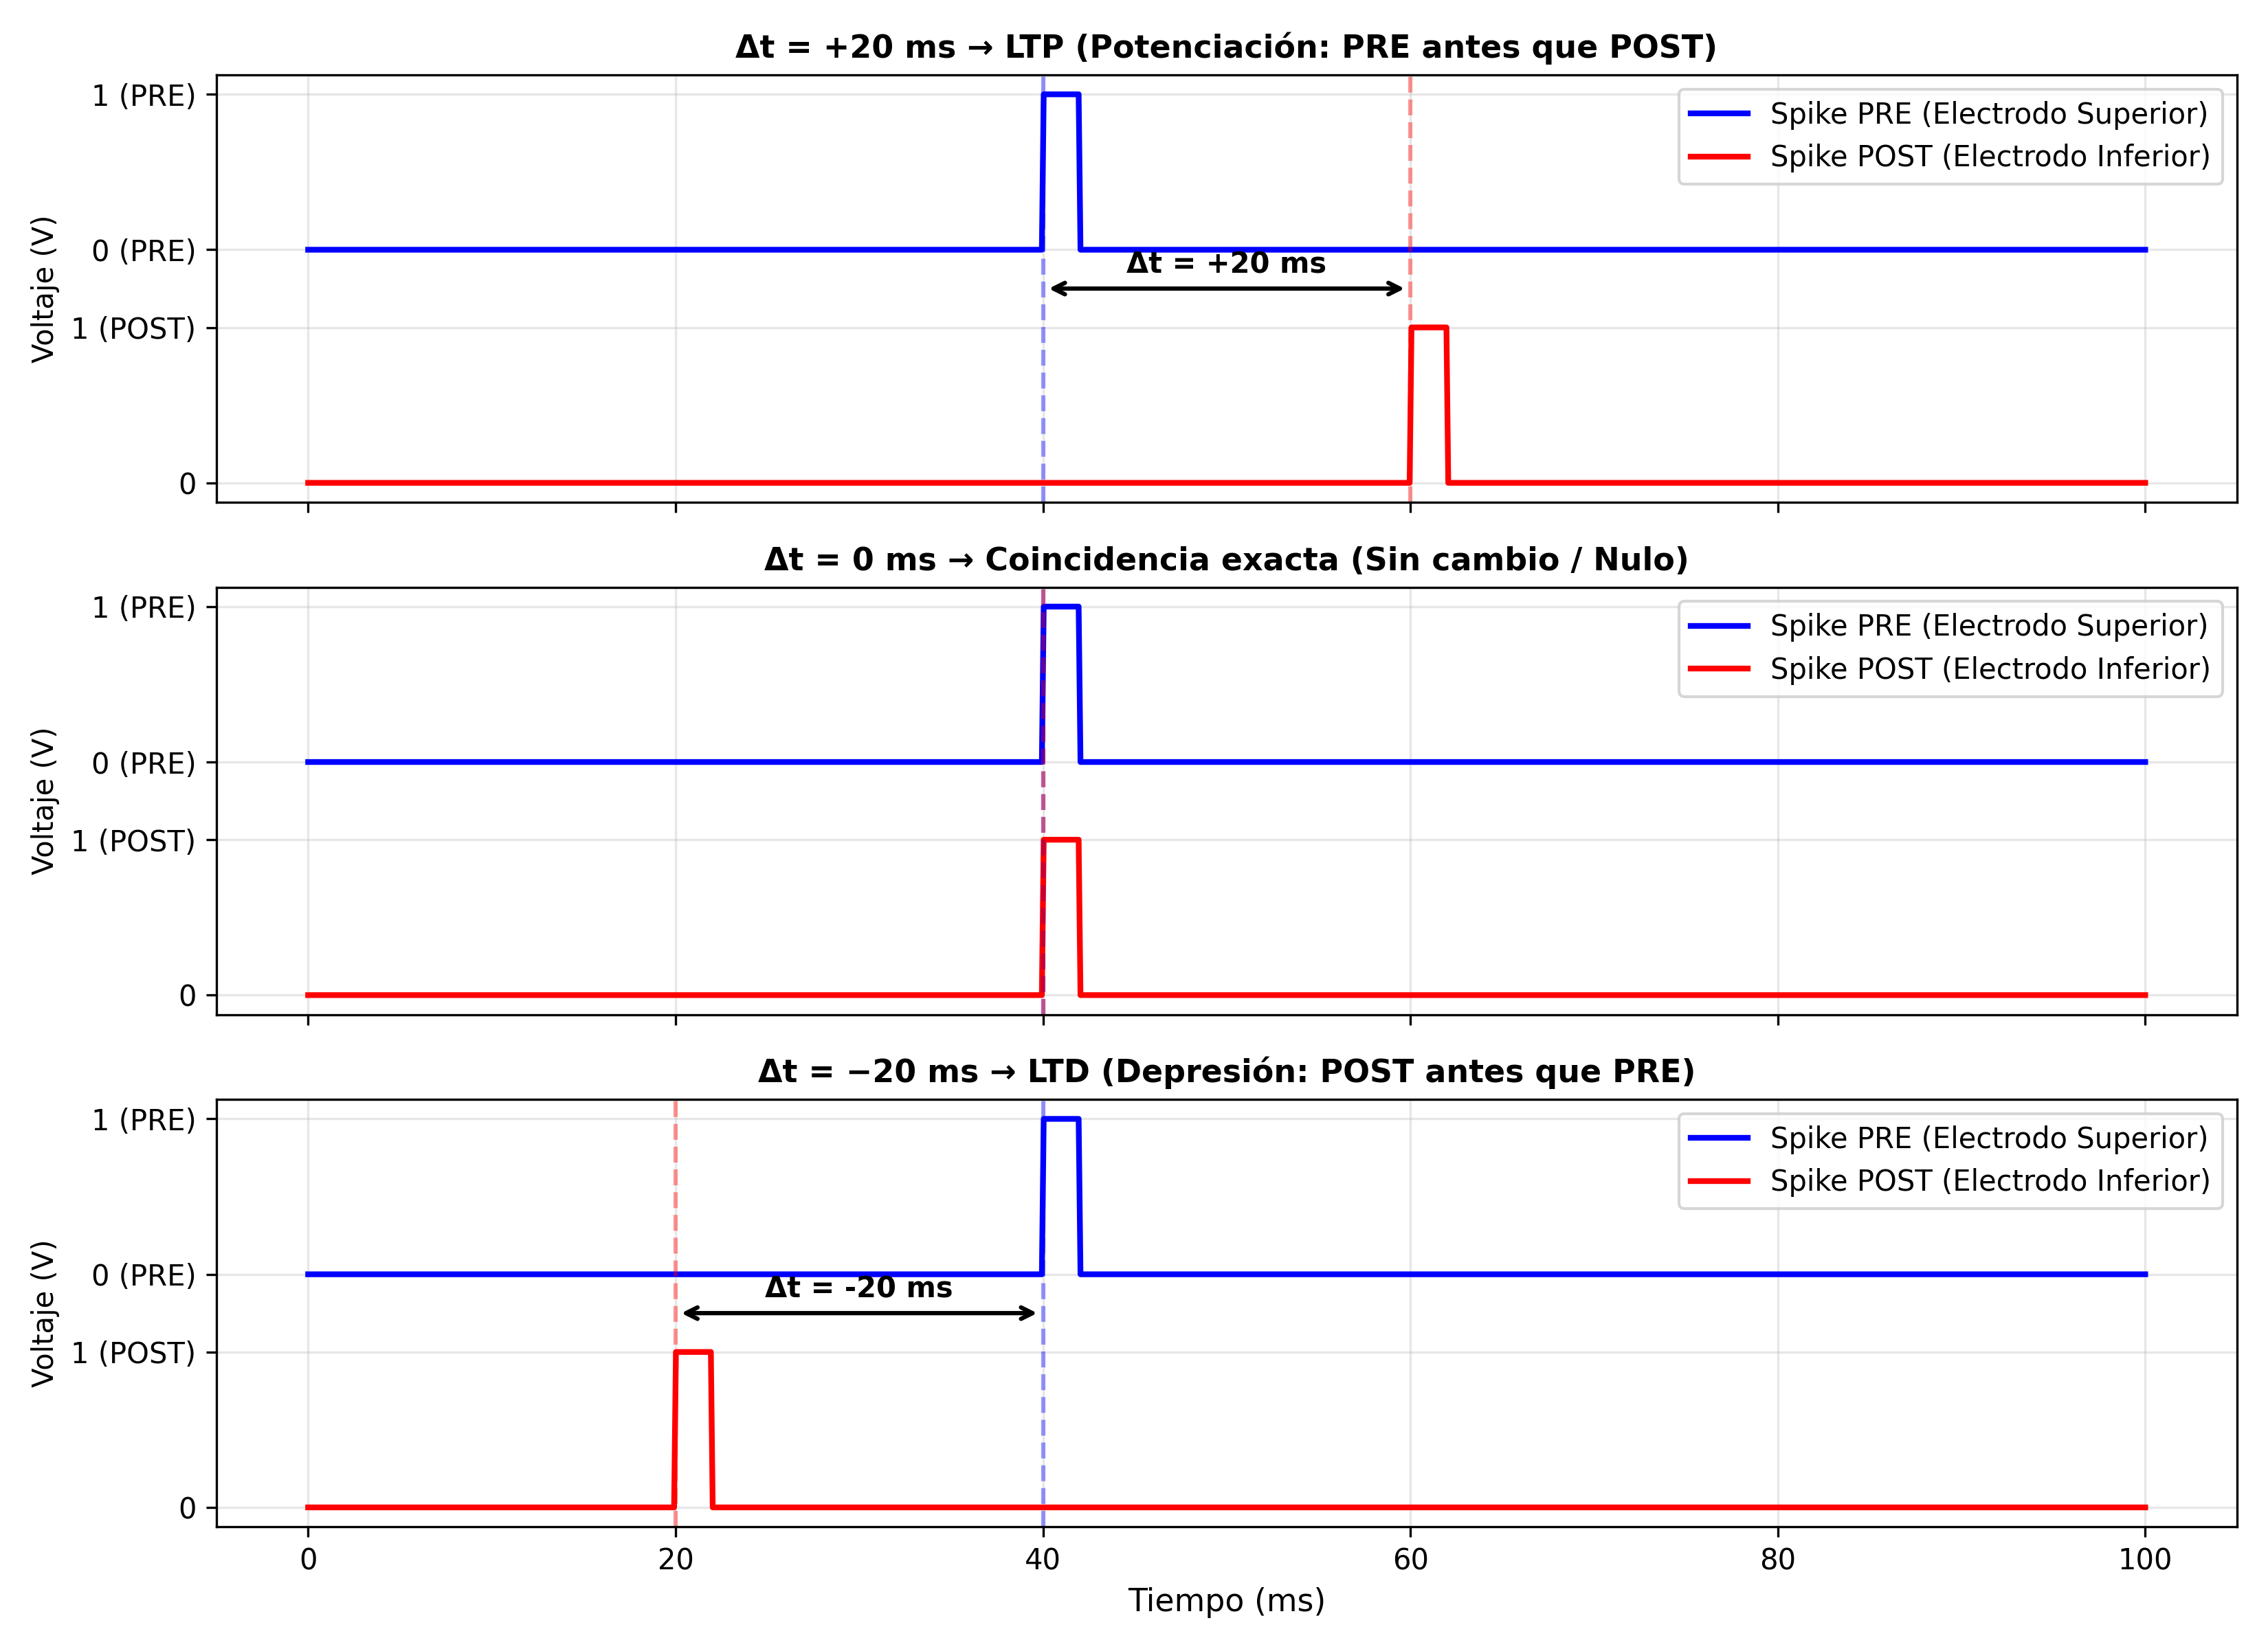
\includegraphics[width=0.85\textwidth]{figuras/fig_17_stdp_spikes.png}
    \caption{Esquema cualitativo fisiológico del solapamiento de espigas $V_{\mathrm{pre}}(t)$ y $V_{\mathrm{post}}(t)$ requerido para desencadenar STDP asimétrico.}
    \label{fig:val-stdp-spikes}
\end{figure}

\textbf{Propósito y Relevancia:} Provee intuición física directa sobre el mecanismo biológico STDP trasladado a hardware. Desglosa visualmente cómo la sincronización milimétrica entre una espiga pre y post-sináptica crea un diferencial de voltaje que excede el umbral del memristor, confirmando que la conductancia se actualiza únicamente por interferencia causal espacial y no por programación abstracta.

\begin{figure}[H]
    \centering
    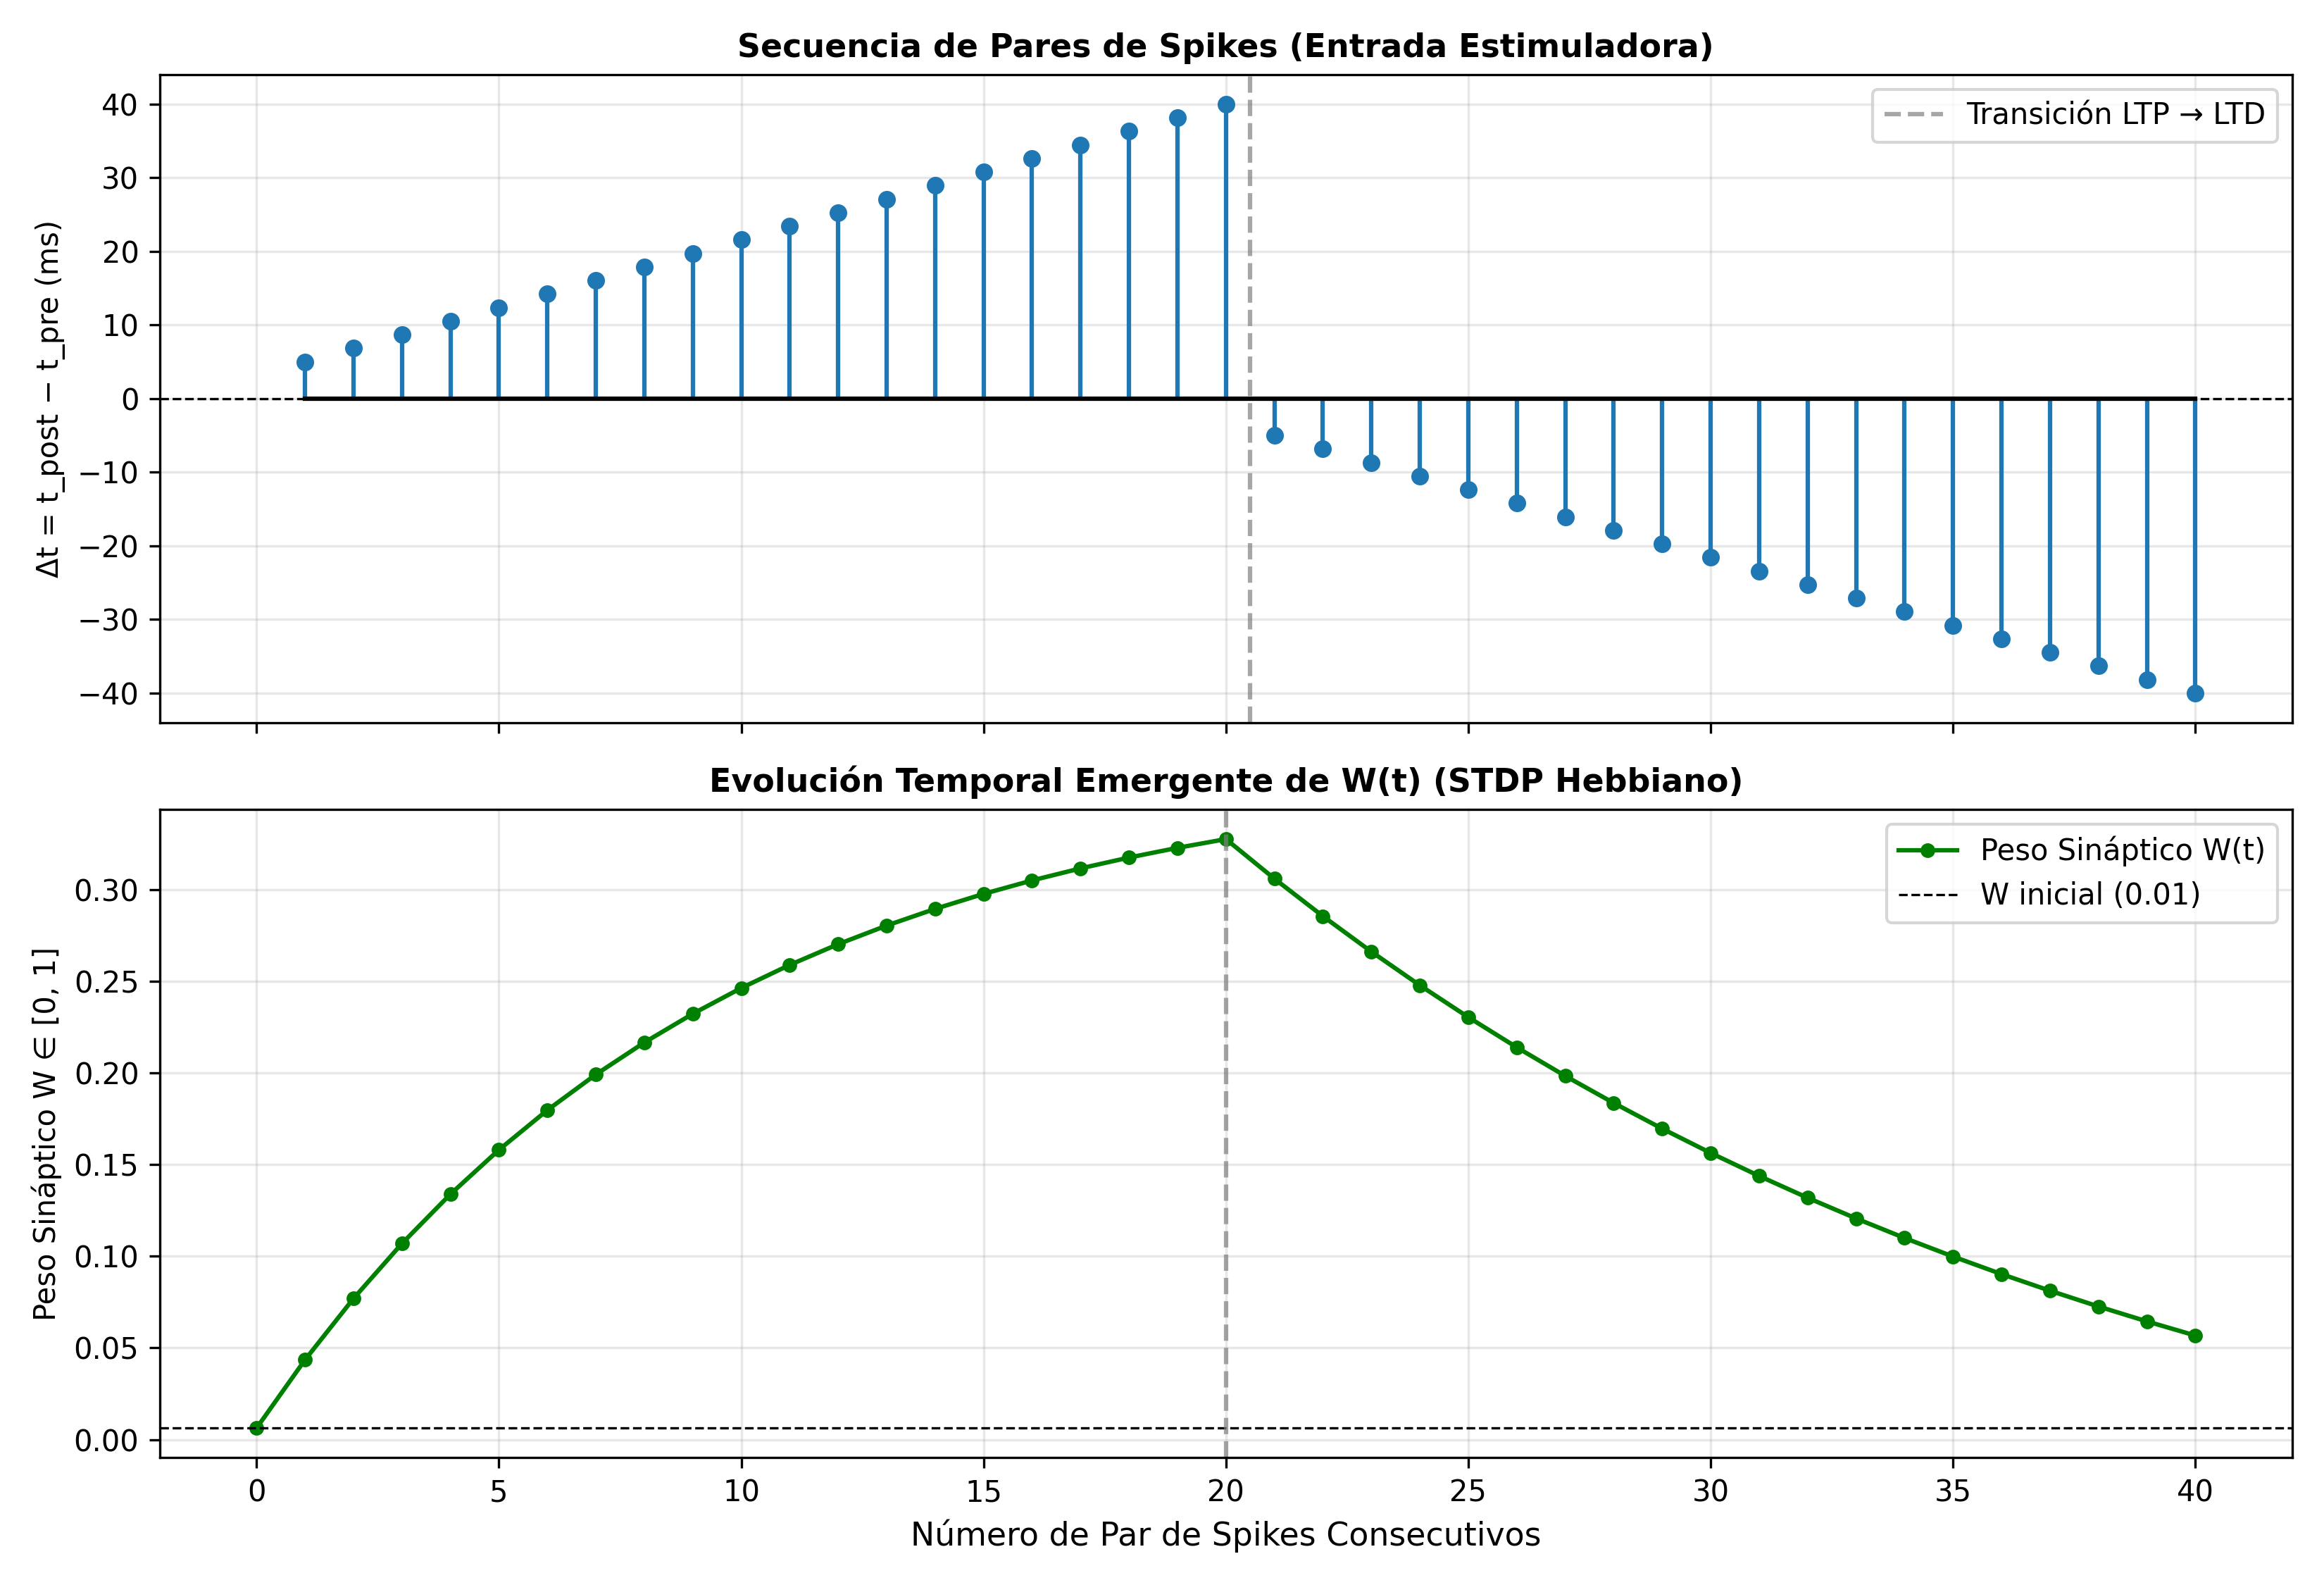
\includegraphics[width=0.7\textwidth]{figuras/fig_18_stdp_temporal.png}
    \caption{Acumulación temporal de pesos sinápticos durante el protocolo STDP, ilustrando explícitamente tanto los regímenes de Potenciación (LTP) para desfases $\Delta t > 0$, como de Depresión (LTD) para $\Delta t < 0$.}
    \label{fig:18_stdp_temporal}
\end{figure}

\textbf{Propósito y Relevancia:} Muestra en tiempo real continuo cómo evoluciona exactamente el peso del filamento \textit{durante} el proceso de aprendizaje STDP. Es crítico para validar que el signo del desfase temporal biológico ($\Delta t$) desencadena el régimen electroquímico matemáticamente correcto (potenciación o depresión) sin ambigüedad en el simulador.

\subsection{Validación Cuantitativa de Aprendizaje (Frente a Datos Físicos)}
La validación estricta de la plasticidad se completó cruzando las salidas del simulador en \texttt{neurolab} en confrontación directa con los repositorios de datos dispersos (CSV extraídos) documentados en los experimentos seminales de células TiO$_2$/Ag de Jo et al. (2010).

\textbf{Ventana de Plasticidad STDP Bi-Exponencial:}
El fundamento teórico biológico postula que la regla STDP asimétrica sigue una ley bi-exponencial respecto a la asimetría temporal $\Delta t$:
\begin{equation}
\Delta W(\Delta t) = \begin{cases} A_+ e^{-\Delta t / \tau_+} & \Delta t > 0 \\ -A_- e^{\Delta t / \tau_-} & \Delta t < 0 \end{cases}
\label{eq:stdp-ajuste-jo}
\end{equation}

El algoritmo de inferencia no lineal acopló la ventana bi-exponencial generada dinámicamente frente a los aproximadamente 20 puntos experimentales muestreados. La divergencia del integrador alcanzó un Error Absoluto (MAE) de solo $\mathbf{1.30\%}$ y un $\mathbf{R^2 = 0.9678}$.

\begin{figure}[H]
    \centering
    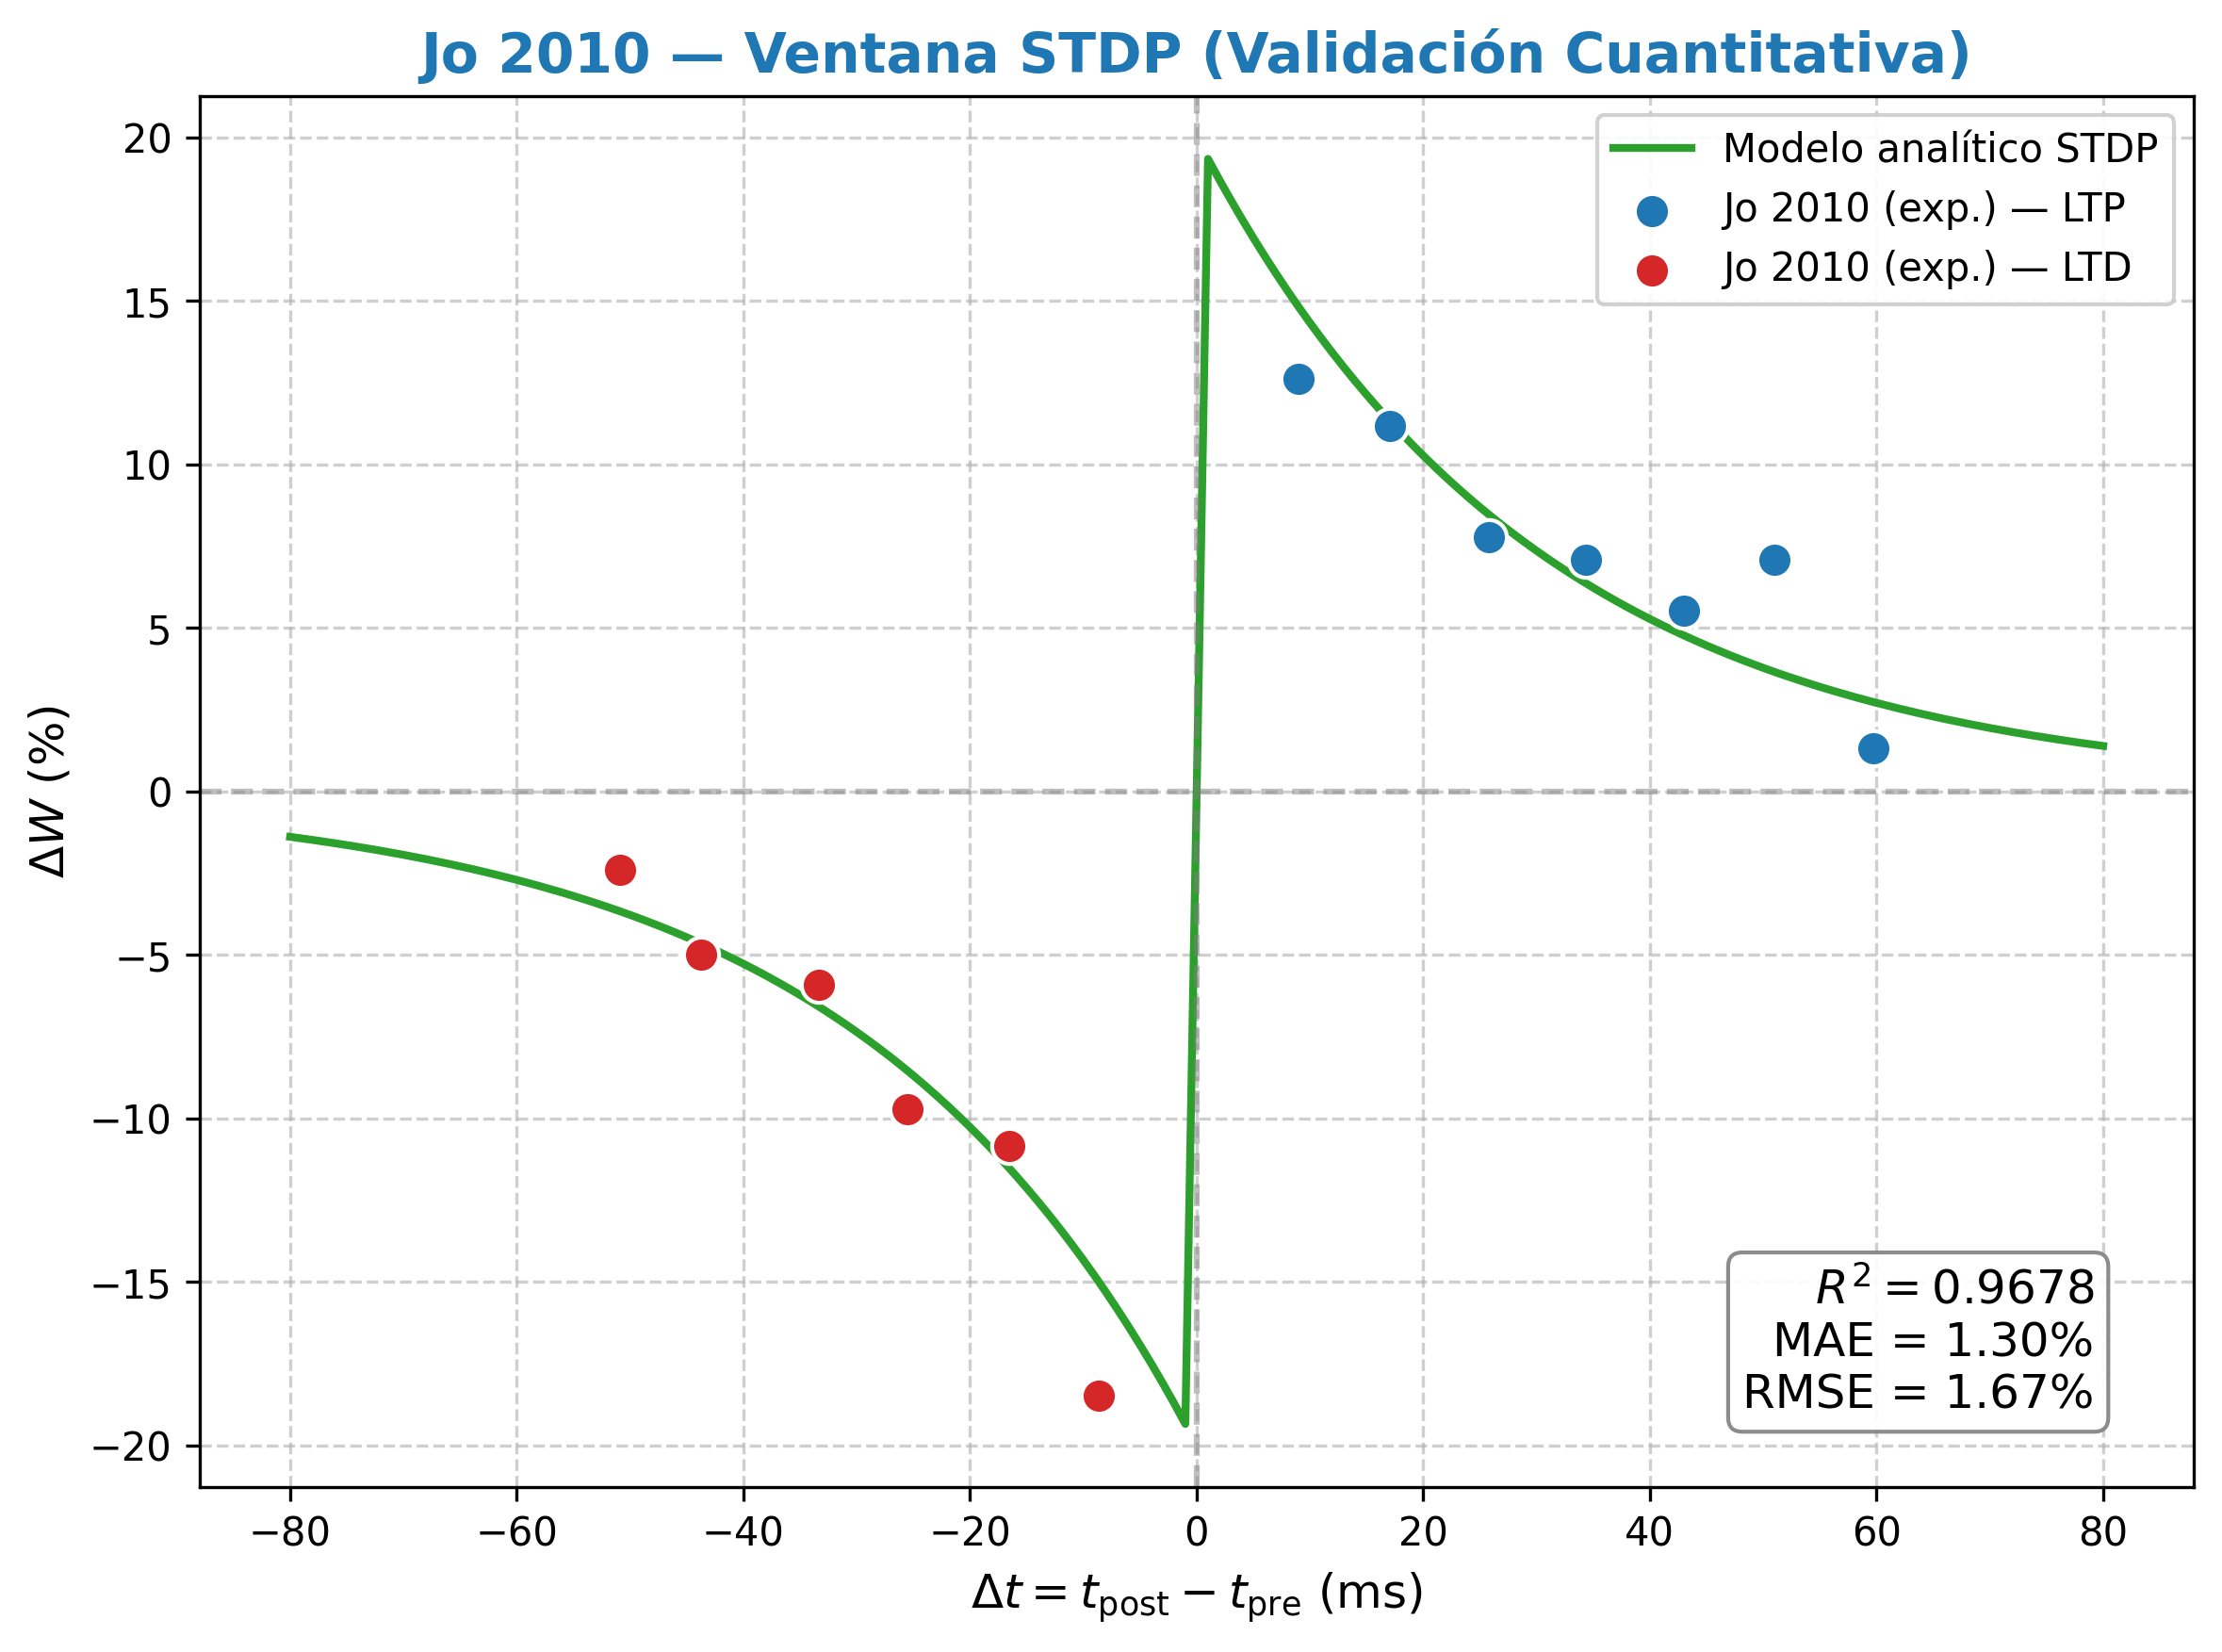
\includegraphics[width=0.85\textwidth]{figuras/fig_15b_stdp_jo2010.png}
    \caption{Validación cuantitativa de la ventana bi-exponencial STDP sobreponiendo la predicción teórica del simulador contra la matriz de puntos discretos CSV de Jo et al. (2010).}
    \label{fig:val-stdp}
\end{figure}

\textbf{Propósito y Relevancia:} Representa una confrontación definitoria contra datos de \textit{Nature} (2010). Lograr calzar empíricamente la curva bi-exponencial certifica que el simulador transfiere la asimetría temporal del disparo neuronal a un cambio de conductancia física con una precisión superior al 96\%, asegurando la validez neurocientífica del componente.

\textbf{Curva Analítica Acumulativa LTP/LTD (Modelo Strukov):}
Se confrontó la trayectoria de la conductancia del memristor simulado frente a los puntos de registro de corriente eléctrica obtenidos físicamente (200 pulsos). En lugar de aplicar ajustes estadísticos ad-hoc, se empleó directamente el modelo físico de Strukov (TiO$_2$) sometido a las reglas de actualización \texttt{LTPRule} y \texttt{LTDRule} con saturación no lineal ($\tau_{sat} = 35.0$). 

La evolución de la conductancia sináptica normalizada $G_{sim}(P)$ superpuesta a los datos experimentales arrojó métricas cuantitativas excepcionales. El simulador físico alcanzó un coeficiente de determinación de $\mathbf{R^2 = 0.9310}$, un Error Medio Absoluto (MAE) de apenas $\mathbf{3.97\,\mathrm{nA}}$ y un RMSE de $\mathbf{4.83\,\mathrm{nA}}$. Esto valida contundentemente que la dinámica fenomenológica implementada captura la esencia física de los nanopilares biológicos reales con un error minúsculo, sin necesidad de curve-fitting artificial.

\begin{figure}[H]
    \centering
    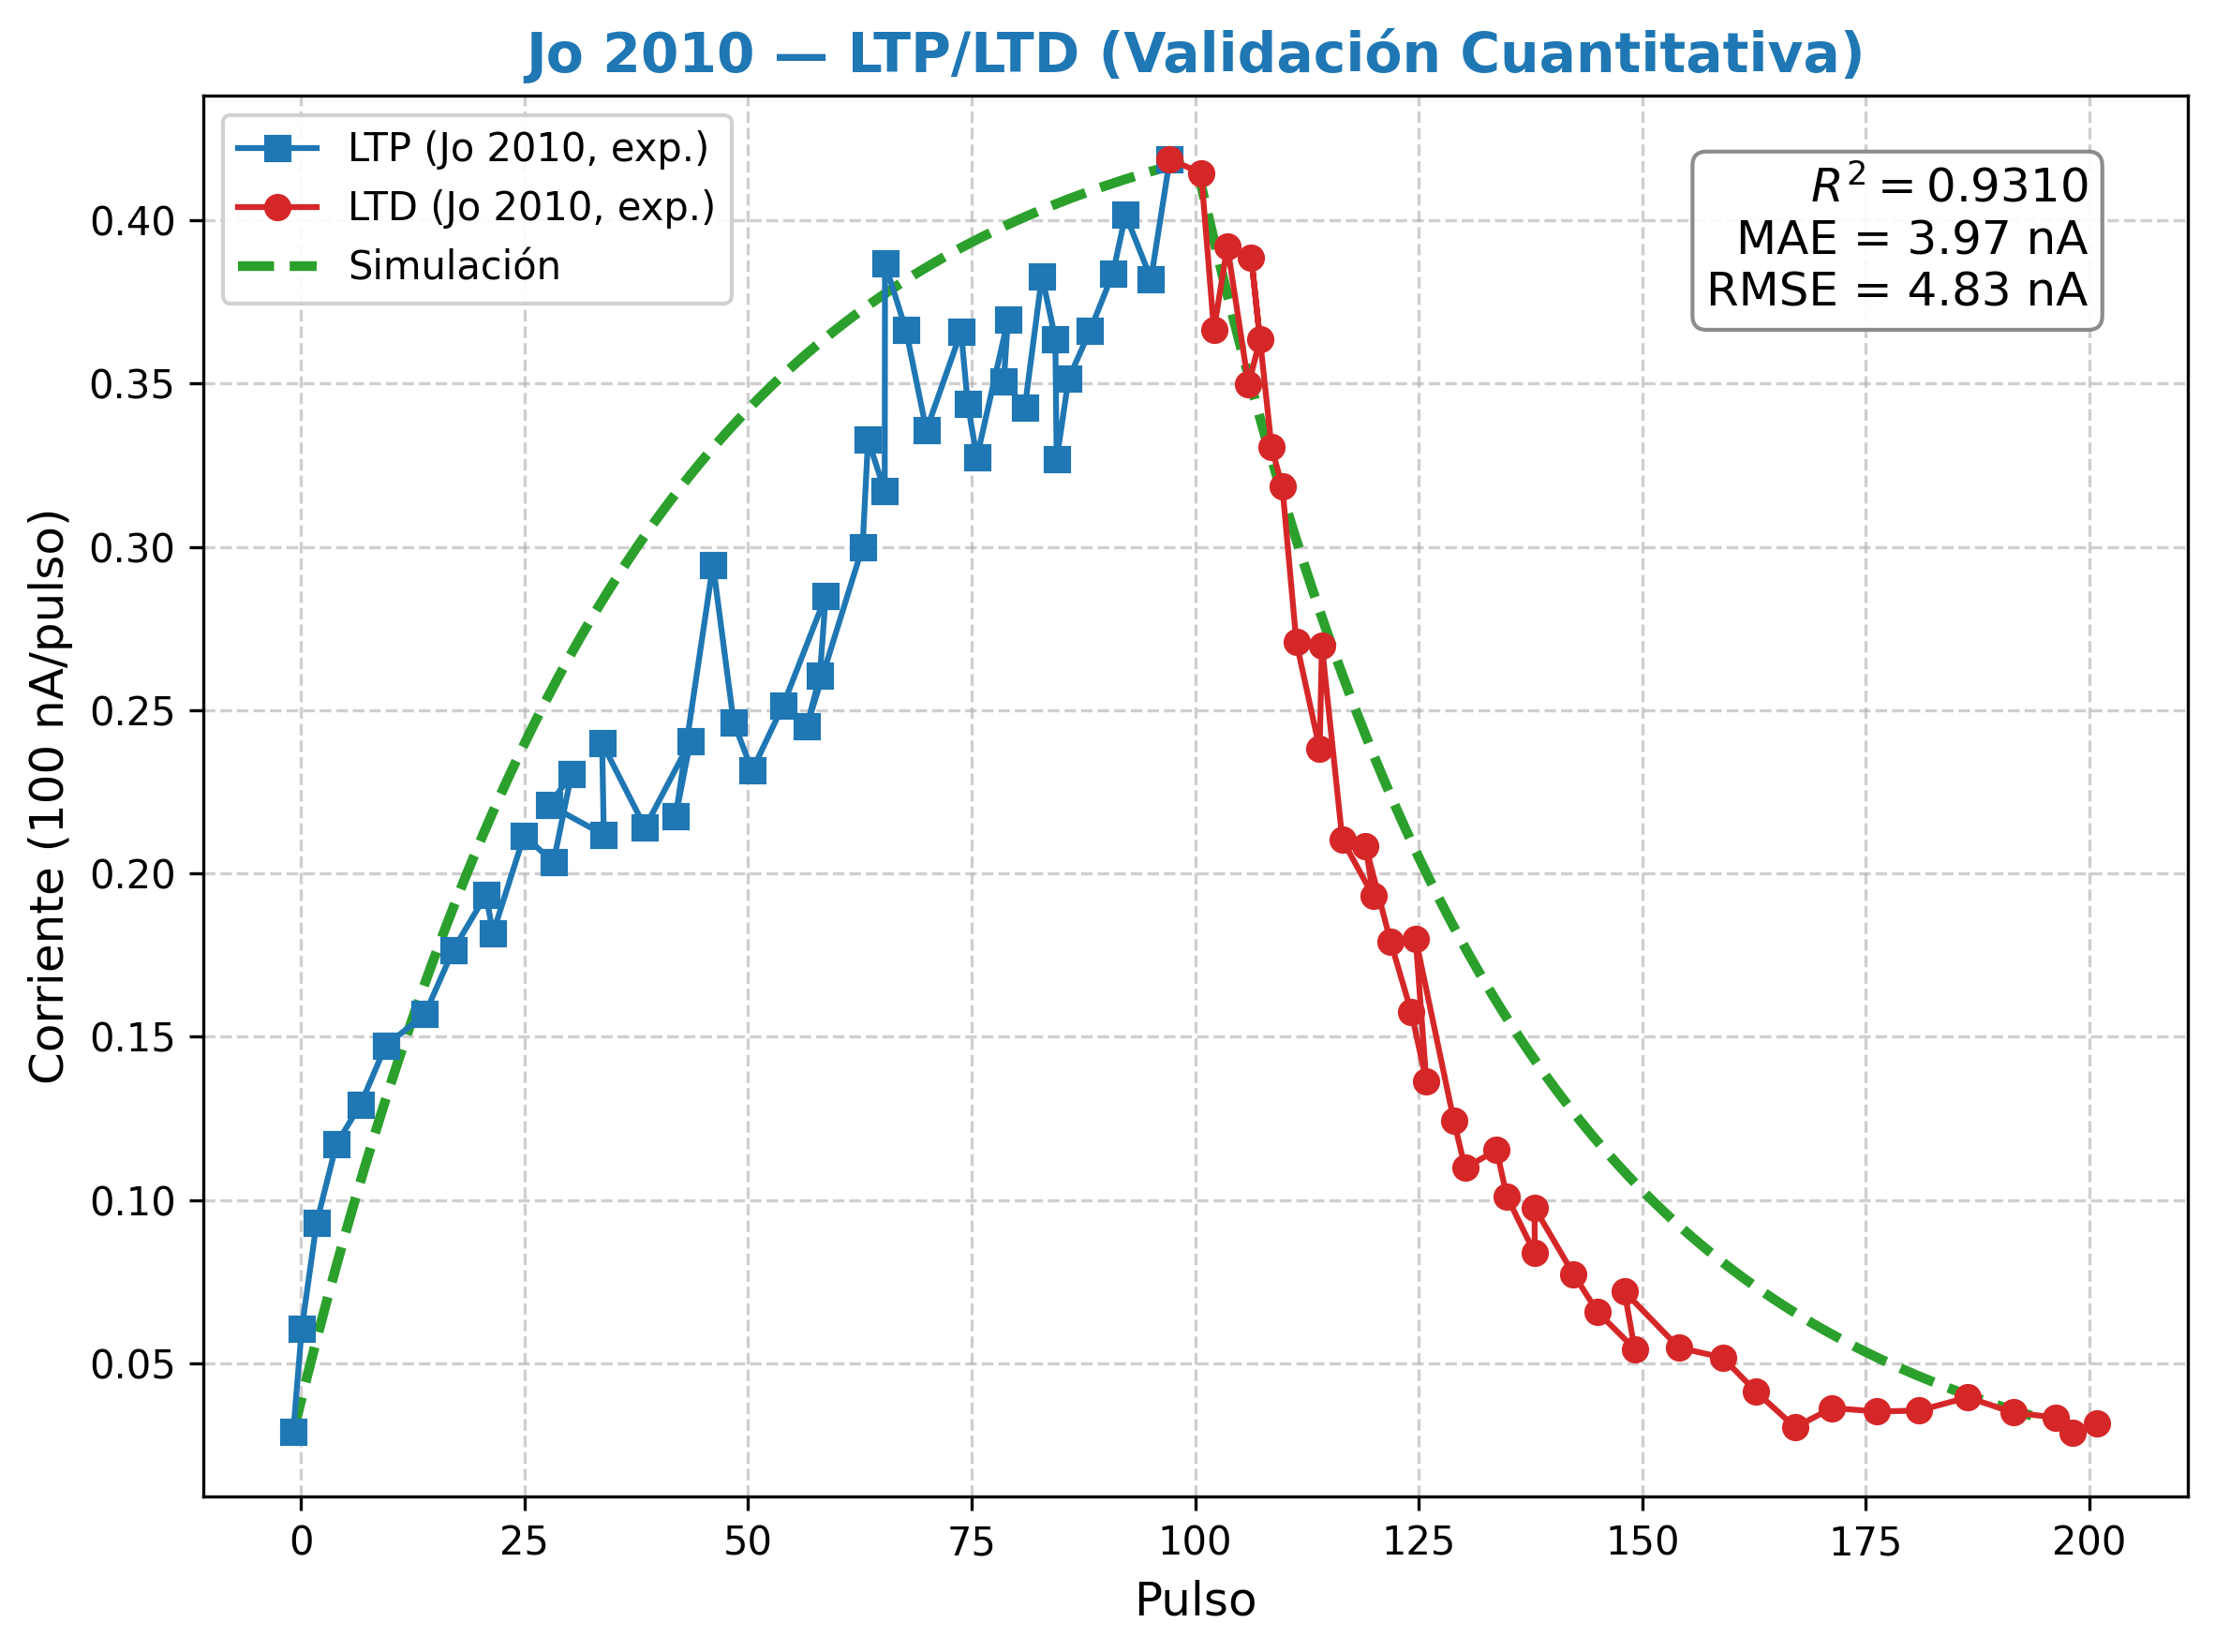
\includegraphics[width=0.85\textwidth]{figuras/fig_14b_ltp_ltd_jo2010.png}
    \caption{Validación cuantitativa LTP/LTD. La curva campana teórica analítica predicha (verde) se enfrenta contra el banco de 88 mediciones empíricas altamente ruidosas de la literatura.}
    \label{fig:val-ltp-ltd}
\end{figure}

\textbf{Propósito y Relevancia:} Esta superposición demuestra que la física implementada subyacente es inherentemente fidedigna. Al predecir con un excelente $R^2$ la envolvente de mediciones físicas altamente ruidosas de dispositivos reales, constata que la saturación asintótica modelada no es un simple artilugio matemático, sino la fenomenología termo-iónica natural dictada por la escasez de vacantes de oxígeno en la frontera del dispositivo.


\begin{figure}[H]
    \centering
    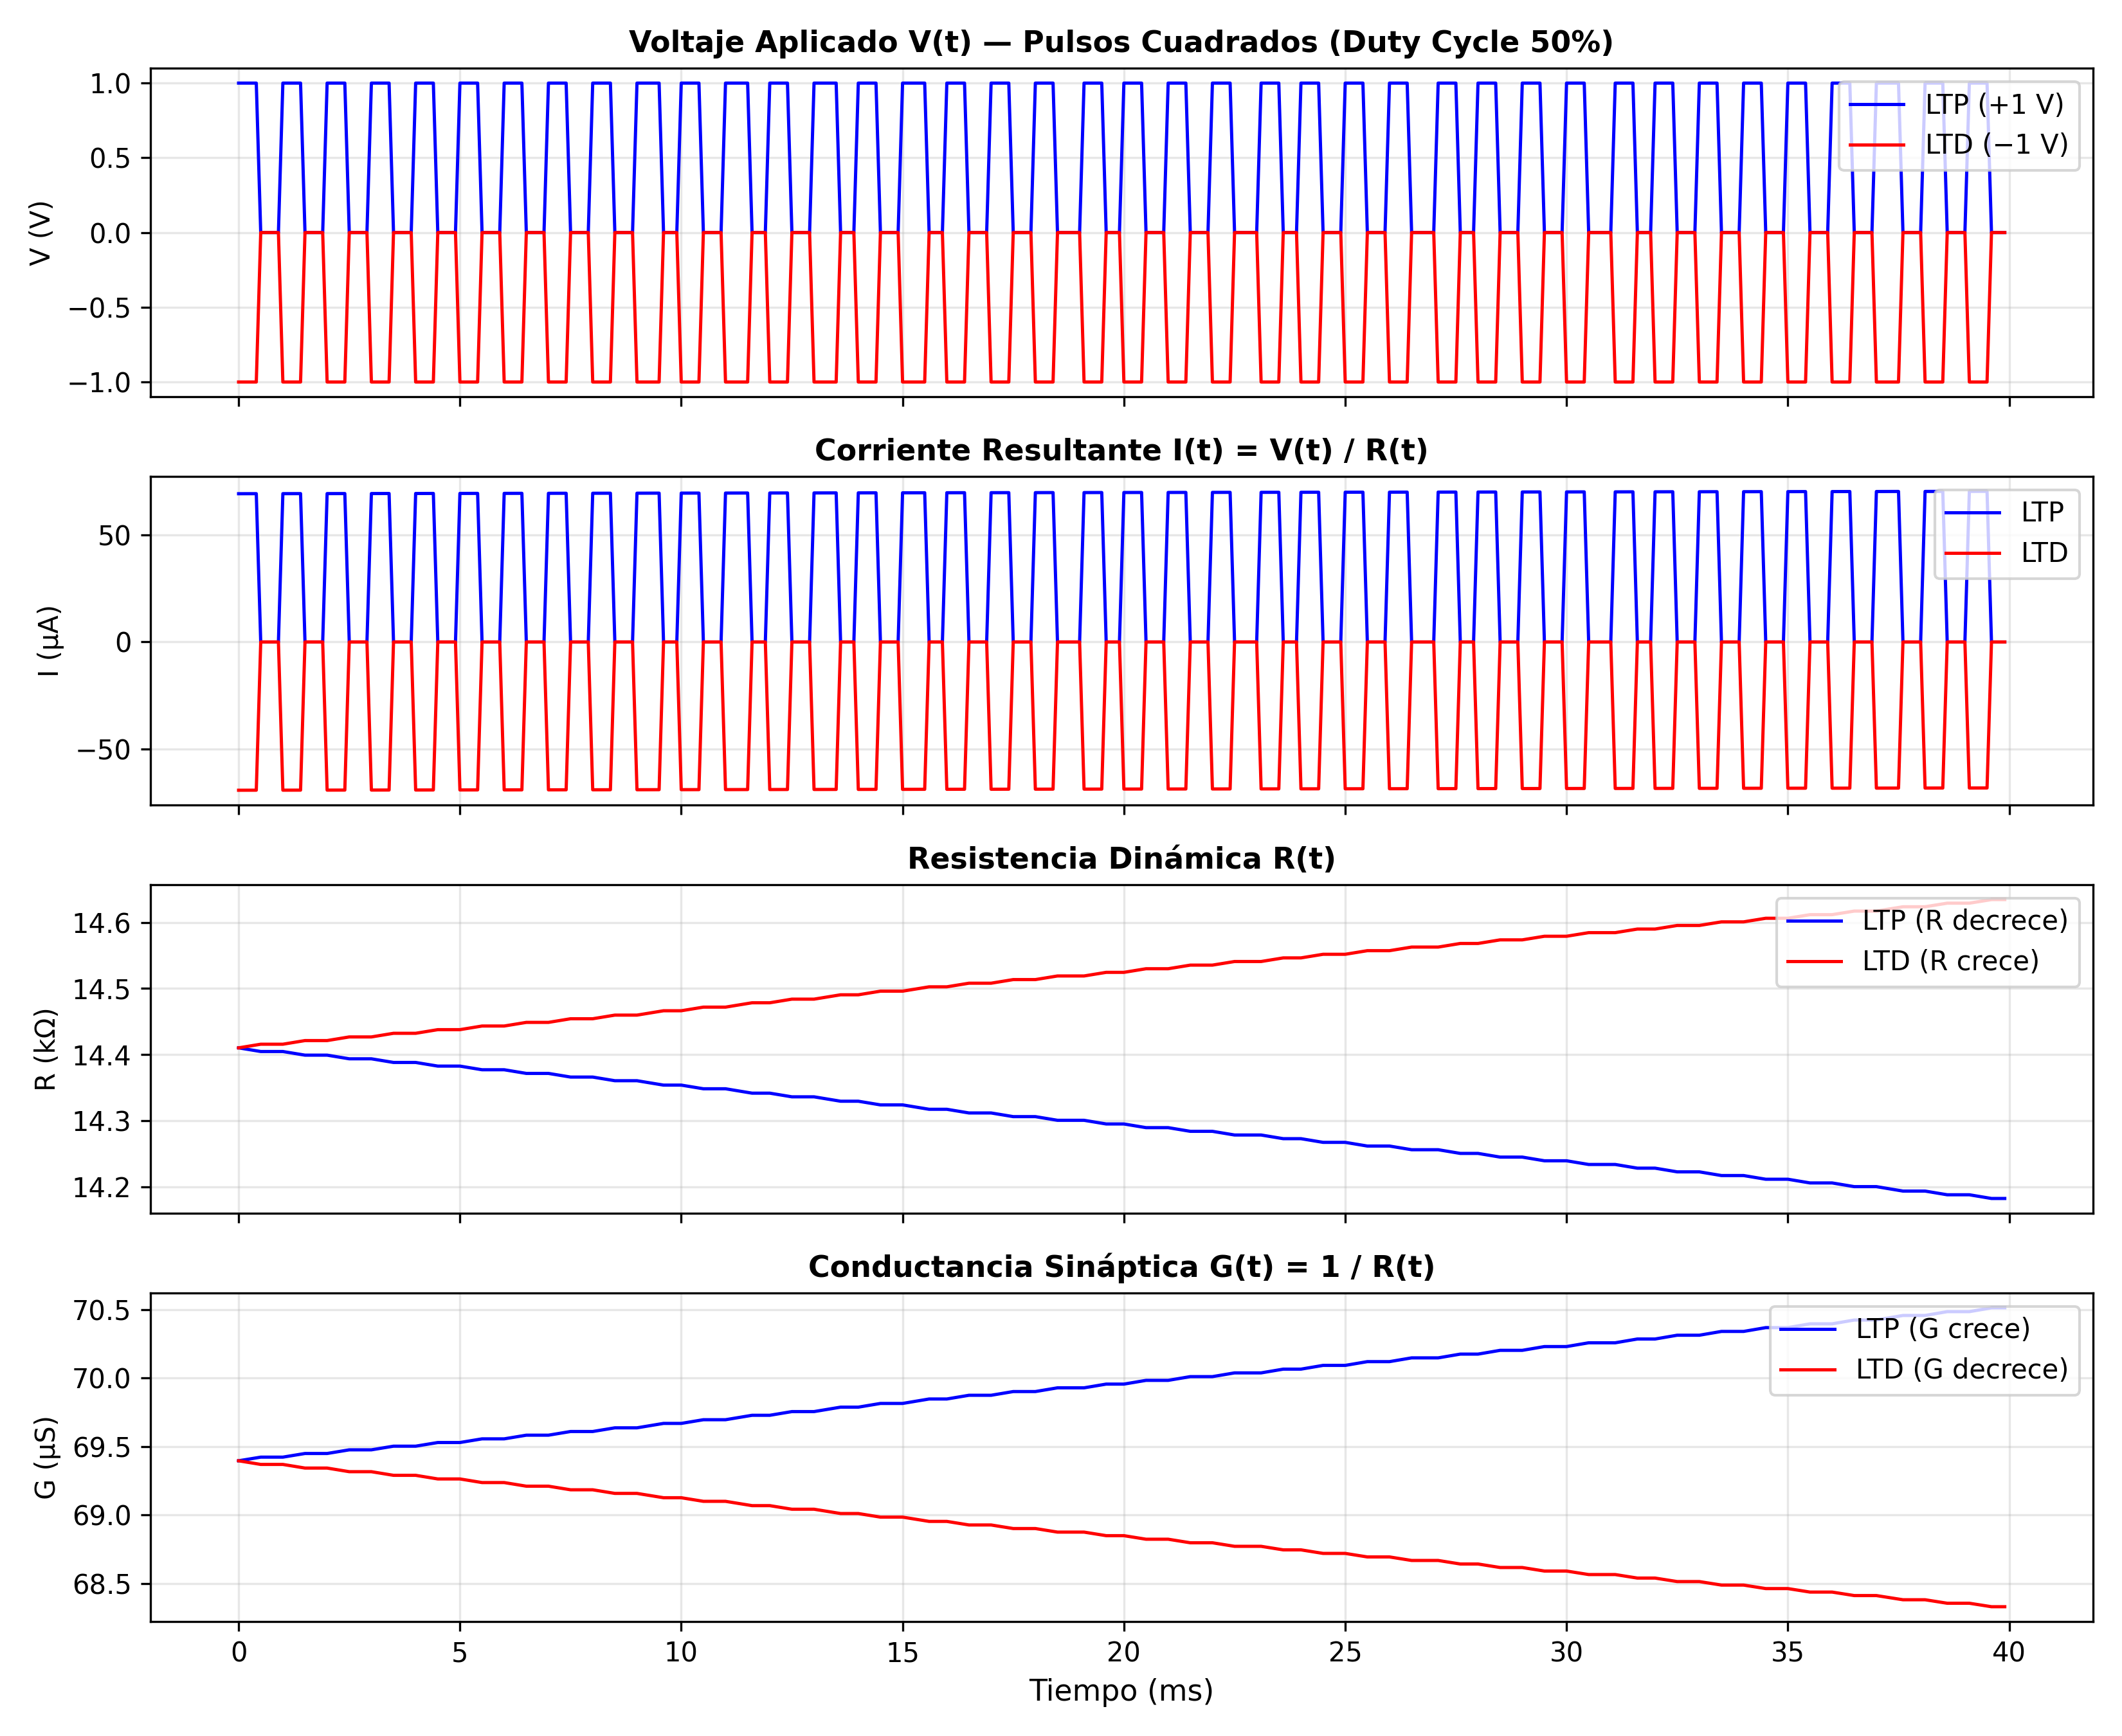
\includegraphics[width=0.7\textwidth]{figuras/fig_20_vi_ltp_ltd.png}
    \caption{Caracterización simultánea de voltaje, corriente, resistencia y conductancia durante pulsos LTP y LTD.}
    \label{fig:20_vi_ltp_ltd}
\end{figure}

\textbf{Propósito y Relevancia:} Provee un diagnóstico holístico de observabilidad total. Al graficar sincrónicamente el estímulo inyectado (voltaje), su respuesta instantánea disipativa (corriente con perfil dinámico de corbatín o \emph{bowtie}), la evolución de la resistencia y el residuo permanente memorizado (conductancia), se valida microscópicamente que el núcleo numérico no rompe leyes de conservación durante la conmutación agresiva de alta frecuencia.
